\chapter{ALGORITMOS PROPOSTOS PARA CONSTRUÇÃO DE FLORESTA DE ÁRVORES ARTERIAIS} \label{sec:algoritmos-propostos}

Neste capítulo, apresenta-se os algoritmos propostos nesta tese para gerar florestas de árvores 
arteriais concorrentes e que não se comunicam.

Diferentemente dos algoritmos apresentados na Seção~\ref{sec:construcao-de-multiplas-arvores}, 
os algoritmos desenvolvidos podem incorporar no processo de geração das florestas 
um controle de invasão das árvores, bem como a geração em estágios de crescimento através 
de uma estratégia baseada no diagrama de Voronoi~\cite{Aurenhammer2004}.

\section{CONSTRUÇÃO DE FLORESTAS DE ÁRVORES ARTERIAIS COM COEFICIENTE DE INVASÃO} \label{sec:floresta-com-invasao}

Para permitir um controle melhor da invasão de uma árvore no território da outra, é proposto 
neste trabalho o Algoritmo~\ref{algo:FlorestaDeArvoresComInvasao} 
(baseado em~\cite{Jaquet2019}). Para obter esse controle, 
em relação à árvore $t$, admite-se o ponto $\mathbf{x}_{inew}$ 
como posição distal de um novo segmento terminal se atender as condições:
\begin{enumerate}[label=(\roman*)]
 \item estiver dentro do domínio de perfusão;
 \item sua distância 
até $\mathbf{x}_{root}^t$ for menor ou igual a $l_{max}^t$ 
(conforme definido em~\eqref{eq:criterio.distancia.raiz}). Essa condição 
só é considerada enquanto o fluxo atual da árvore $t$ for menor ou igual a $\alpha q^t_{targ}$, 
onde $\alpha\in[0,\,1]$ é um coeficiente constante de invasão. Quanto mais próximo $\alpha$ estiver de $1$, menos 
uma árvore invade o território vascular da outra;
 \item sua distância a todos os segmentos da árvore $t$ for maior do que 
 \begin{equation}
   d_{min} = \sqrt[n]{\dfrac{|D_{perf}|}{K_{term}}}
   \label{eq:distancia-minima}
 \end{equation}
 onde $n = 2$ (no caso bidimensional) ou 
 $n = 3$ (no caso tridimensional), $|D_{perf}|$ é a área de $D_{perf}$ (ou o volume, conforme valor de $n$)
 e $K_{term}$ é a soma do número de segmentos terminais de todas as árvores no passo atual. Nota-se que 
 geometricamente $d_{min}$ vai representar o lado do quadrado (ou aresta do cubo) de uma unidade 
 de área (ou unidade de volume) delimitada por $D_{perf}$.
\end{enumerate}

A Figura~\ref{fig:passos-metodo-proposto} ilustra o funcionamento básico do Algoritmo~\ref{algo:FlorestaDeArvoresComInvasao}.

\begin{algorithm}
  \Dados{
    $D_{perf}$, $\mathbf{x}_{root}^t$, $q_{targ}^t$, $N_{term}$,
    $N_{con}$, $N_{trees}$, $\eta$, $\alpha$, $\beta$.
  }
  Gerar e validar uma posi\c{c}\~ao distal $\mathbf{x}_{inew}^t$ do 
  segmento raiz da árvore $t=1,\,2,\,\ldots,\,N_{tree}$, respeitando a distância 
  $l_{max}^t$\;
  Conectar $\mathbf{x}_{inew}^t$ a $\mathbf{x}_{root}^t$ (\textit{plantar o segmento raiz da árvore }$t$)\;
  \For{($K_{term}\gets 1$ \KwTo $N_{term}$)}{
    Marcar as árvores como ativa ou inativa, baseado no seu fluxo atual\;
    Gerar a posi\c{c}\~ao distal $\mathbf{x}_{inew}$ de um novo segmento terminal e 
    verificar as condições (i), (ii) e (iii)\;
    Determinar $N \leq N_{con}$ segmentos que estão mais próximos de $\mathbf{x}_{inew}$ nas 
    árvores ativas\;
    \For{($j\gets 0$ \KwTo N)}{
      Conectar $\mathbf{x}_{inew}$ temporariamente no segmento $j$, 
      criando a bifurca\c{c}\~ao $\mathbf{x}_{ibif}$\;
      Otimizar e validar a posi\c{c}\~ao de $\mathbf{x}_{ibif}$\;    
      Armazenar resultados de $\mathbf{x}_{ibif}$ na TAC\;
      Descartar conexão temporária $\mathbf{x}_{ibif}$\;
    }
    Obter TAC$_r$ a partir de TAC removendo as conexões inválidas\;
    Determinar em TAC$_r$ a bifurcação ótima $\mathbf{x}_{iopt}$\;
    Conectar $\mathbf{x}_{inew}$ a $\mathbf{x}_{iopt}$ de modo permanente\;
  }
\caption{Gera\c{c}ão de floresta de árvores arteriais com coeficiente de invasão.}
\label{algo:FlorestaDeArvoresComInvasao}
\end{algorithm}

\begin{figure}[!htb]
  \centering
  \captiondelim{: }
  \caption{Ilustração dos passos básicos do Algoritmo~\ref{algo:FlorestaDeArvoresComInvasao} no crescimento 
    de uma floresta com $N_{trees} = 2$. 
    (a) O ponto $\mathbf{x}_{inew}$ é escolhido aleatoriamente dentro do domínio de perfusão. 
    Testa-se a conexão desse ponto com os $N \leq N_{con}$ segmentos mais próximos 
    nas árvores ativas. Será feita permanente a conexão que fornecer o menor volume total. 
    (b) Exemplo do teste de conexão do ponto $\mathbf{x}_{inew}$ com
    um segmento próximo na árvore 1.
    (c) Exemplo do teste de conexão do ponto $\mathbf{x}_{inew}$ com
    um segmento próximo na árvore 2.
  }
  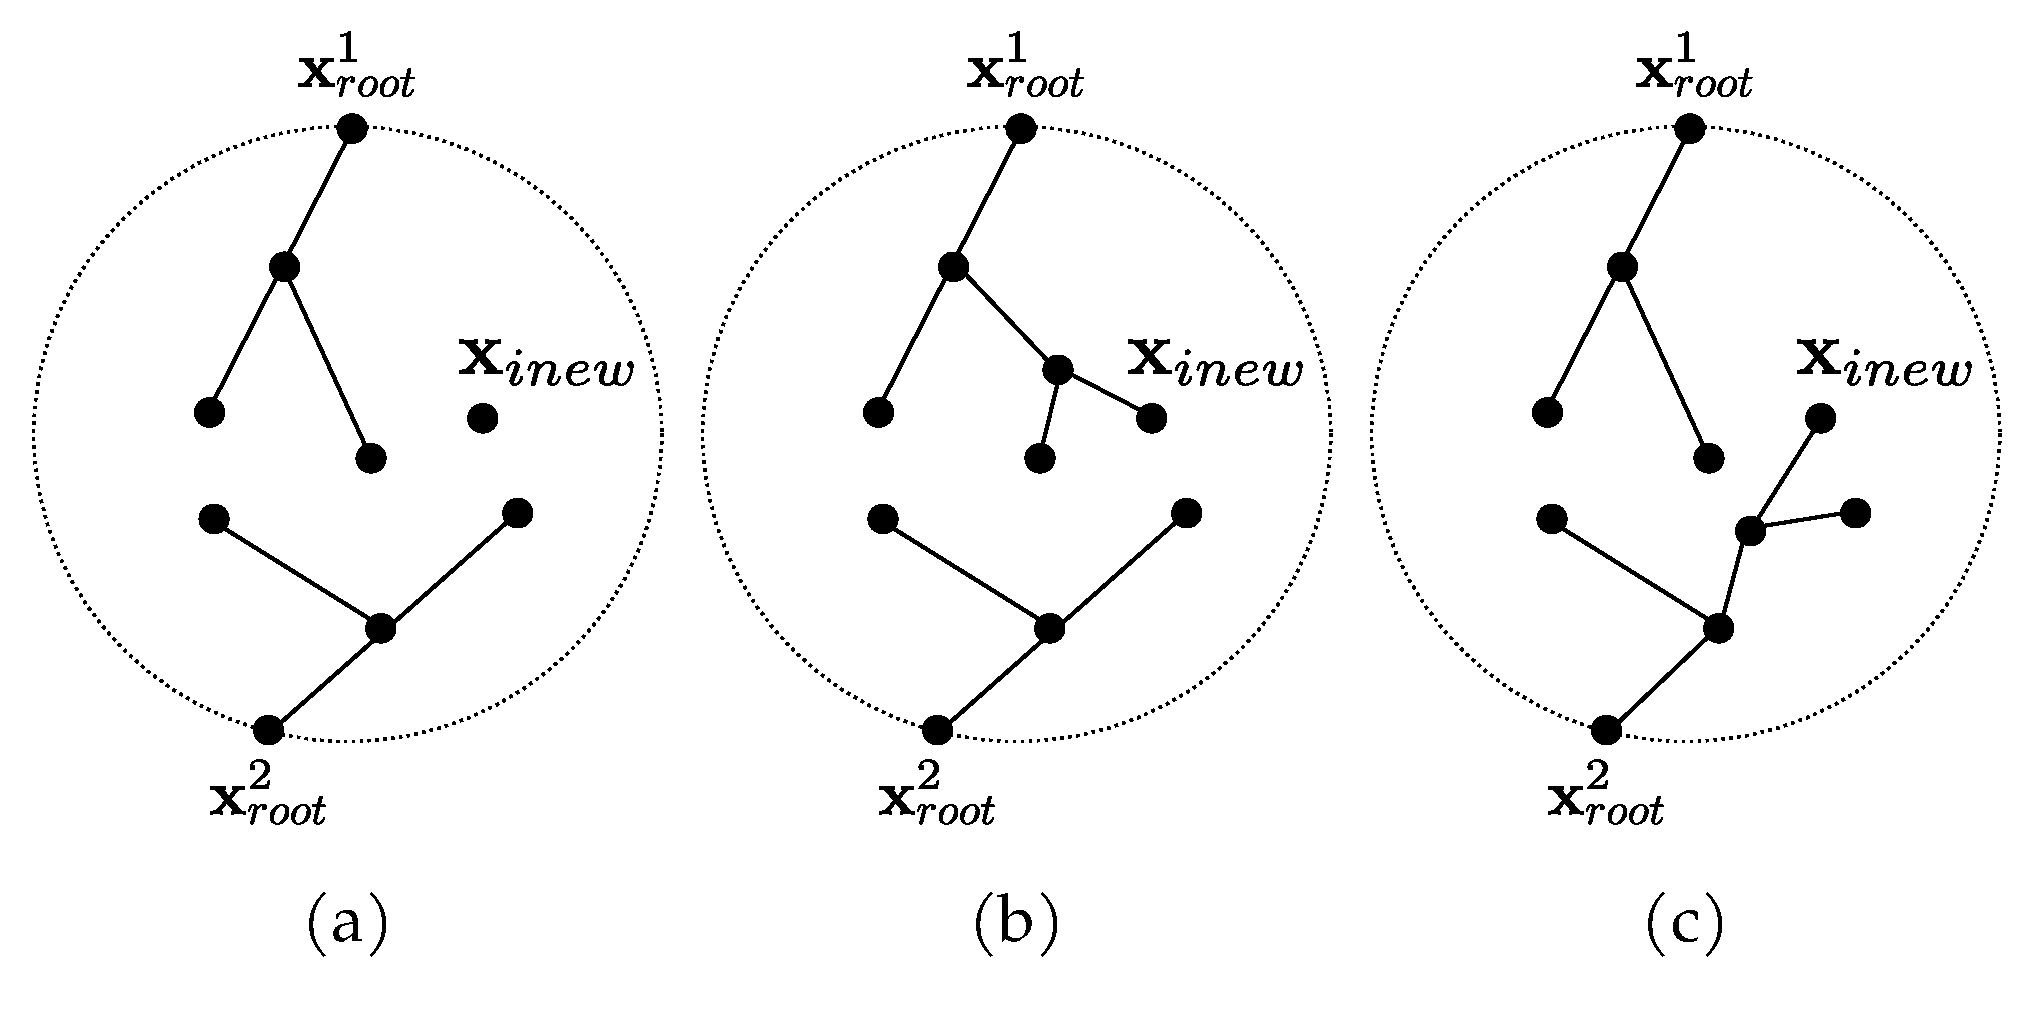
\includegraphics[scale=0.4]{figuras/modelos-computacionais-de-arvores-circulatorias/passos-algoritmo-cco-narvores.eps}
  \fonteAutor{2022}
  \label{fig:passos-metodo-proposto}
\end{figure}

Para otimizar a posição $\mathbf{x}_{ibif}$ na iteração mais
interna do Algoritmo~\ref{algo:FlorestaDeArvoresComInvasao}, utilizou-se a 
estratégia de mapeamento~\eqref{eq:mapeamento-bifucacao} como mencionada na 
Seção~\ref{subsec:arvores-arterial-venosa}.

Conforme explicado na Seção~\ref{subsec:floresta-vascular}, o ponto $\mathbf{x}_{inew}$ será 
válido somente se o segmento mais próximo dele estiver em uma 
árvore ativa. Caso necessário, deve-se gerar aleatoriamente outras posições 
até que $\mathbf{x}_{inew}$ seja válido. O critério de distância presente na 
condição (iii) pode ser muito restritivo e o processo aleatório de geração pode 
ser repetido muitas vezes. Para relaxar esse critério, 
se a geração de $\mathbf{x}_{inew}$ for repetida $N_{toss}$ vezes sem conseguir 
obter uma posição que atenda (iii), então $d_{min}$ será atualizado como 
$\beta d_{min}$, onde $\beta\in (0,\,1)$ é um fator de redução. Além disso, 
$d_{min}$ também será atualizado se por $N_{toss}$ vezes a posição atender 
(iii), mas não for possível obter uma bifurcação ótima $\mathbf{x}_{iopt}$.

\section{CONSTRUÇÃO DE FLORESTAS DE ÁRVORES ARTERIAIS EM ESTÁGIOS} \label{sec:coat}

O algoritmo proposto na Seção~\ref{sec:floresta-com-invasao} utiliza a estratégia de 
modificar o método CCO de modo a construir mais de uma árvore simultaneamente 
sem subdividir o domínio de perfusão. Por outro lado, para explorar a estratégia de 
subdividir o domínio de perfusão e construir cada árvore da floresta no seu respectivo
subdomínio, nesta seção é proposto um algoritmo chamado \textit{Competing Optimized Arterial Trees} 
(COAT) que é baseado no método CCO.

Suponha que deseja-se construir $N_{trees}$ árvores binárias em um domínio de perfusão $D_{perf}$, 
cada uma com um fluxo alvo $q_{targ}^t$, onde $t = 1,\,2,\,\ldots,\,N_{trees}$.
Durante o crescimento da floresta é criado uma competição entre as 
árvores para ocupar o domínio $D_{perf}$. Para isso, é analisado o fluxo relativo entre elas
(conforme~\eqref{eq:fluxo.relativo.temporario} e~\eqref{eq:fluxo.relativo.total}).

O Algoritmo~\ref{algo:COAT} representa o COAT. Ele 
gera uma floresta de árvores circulatórias em dois estágios. 
No primeiro estágio, o domínio de perfusão será ocupado por 
uma floresta inicial. 
Essa floresta inicial pode ser construída automaticamente durante esse estágio 
conforme Seção~\ref{subsec:construcao-floresta-inicial}. Além disso, esta floresta inicial 
pode ser obtida através da reconstrução de imagens médicas de tomografia 
computadorizada, por exemplo. Inicialmente, essa floresta pode ainda ser gerada 
empregando o algoritmo proposto de controle de invasão descrito na Seção~\ref{sec:floresta-com-invasao}.

Em seguida, a floresta 
inicial é usada para dividir o domínio de perfusão em subdomínios 
disjuntos, cada um associado a uma das árvores.
No segundo estágio, as árvores na floresta continuarão 
o seu crescimento dentro do seu respectivo subdomínio.

\subsection{Construção automática da floresta inicial no primeiro estágio}\label{subsec:construcao-floresta-inicial}

Uma maneira de construir a floresta inicial durante o primeiro estágio pode 
ser conforme explicado a seguir. Inicialmente, são gerados aleatoriamente 
pontos $\mathbf{x}_{inew}^t$ que serão candidatos a ponto distal 
dos segmentos raízes das árvores. Cada ponto $\mathbf{x}_{inew}^t$ é 
considerado válido se estiver dentro do domínio de perfusão e se sua distância ao 
ponto $\mathbf{x}_{root}^t$ (ponto proximal do segmento raiz da árvore $t$) for 
menor ou igual a $l_{max}^t$ (conforme definido em~\eqref{eq:criterio.distancia.raiz}).
Após esta etapa de geração e validação, 
o ponto $\mathbf{x}_{inew}^t$ será conectado ao ponto $\mathbf{x}_{root}^t$ formando
o segmento raiz da árvore $t$.

Em seguida, serão adicionados mais terminais em cada árvore $t$ na floresta.
Admite-se o ponto $\mathbf{x}_{inew}$ 
como posição distal de um novo segmento terminal se ele atender as condições:
\begin{enumerate}[label=(\roman*)]
 \item estiver dentro do domínio de perfusão;
 \item sua distância 
até $\mathbf{x}_{root}^t$ for menor ou igual a $l_{max}^t$ 
(conforme definido em~\eqref{eq:criterio.distancia.raiz});
 \item sua distância a todos os segmentos da árvore $t$ for maior do que 
 $d_{min}^t$ (conforme definido em ~\eqref{eq:distancia-minima}).
\end{enumerate}

Quando o fluxo da árvore $t$ for igual a $\alpha q_{targ}^t$, onde 
$\alpha\in(0,1)$ é chamado de coeficiente de estágio,
ela será marcada como inativa e deixará de receber novos segmentos terminais.
A construção da floresta inicial estará finalizada quando todas as suas árvores
estiverem marcadas como inativas.

\subsection{Divisão do domínio de perfusão}\label{subsec:divisao-do-dominio-de-perfusao}

Após o primeiro estágio, o domínio de perfusão $D_{perf}$ é dividido em subdomínios 
disjuntos $D_1$, $D_2$, \ldots, $D_{N_{trees}}$. Para efetuar esse processo uma 
estratégia baseada na ideia do diagrama de Voronoi~\cite{Aurenhammer2004} é utilizada,
considerando como pontos de referência os pontos distais dos segmentos da árvore $t$.
Suponha que $P_{cn}^t$ seja o ponto distal na árvore $t$ que está mais próximo de um ponto $P$ do
domínio de perfusão. O subdomínio $D_t$ será composto pelos pontos 
$P$ tais que:
\begin{equation}
  \begin{cases}
	\mathrm{dist}(P,\,P_{cn}^t) < \mathrm{dist}(P, P_{cn}^k),\, \forall k\neq t;\,\textrm{ se }\mathrm{dist}(P,\,P_{cn}^t) < \lambda\max \mathrm{dist}(P, P_{cn}^k)\\
	q_{targ}^t < q_{targ}^k,\, \forall k\neq t;\,\textrm{ caso contr\'ario}\\
  \end{cases},
  \label{def:diagrama-voronoi-coat}
\end{equation}
onde $\lambda\in(0, 1]$ é um peso. Quanto mais próximo de 0 é esse peso, 
mais os fluxos alvo são priorizados durante a subdivisão. Por outro lado, quanto
mais próximo 1, mais será priorizado a distância entre os pontos $P$ e $P_{cn}^t$.

A Figura~\ref{fig:exemplo-construcao-diagrama-voronoi} ilustra um exemplo para determinar 
se um ponto $P$ do domínio de perfusão $D_{perf}$ pertence à região $D_1$ ou $D_2$,
considerando que $\lambda = \dfrac{1}{2}$ e na floresta há duas árvores com $q_{targ}^1 < q_{targ}^2$.
A ideia básica nessa estratégia de divisão é que sempre que um ponto 
$P$ está suficientemente próximo de uma árvore $t$, então ele estará no subdomínio
$D_t$. Entretanto, quando um ponto $P$ está aproximadamente equidistante
de todas as árvores, então o ponto $P$ estará no subdomínio $D_t$ que tem
o menor fluxo alvo ($q_{targ}^t$). Isso ajuda a aumentar o território ocupado pela
árvore com menor fluxo. Caso contrário, esse território ficaria
menor do que o desejado.

\clearpage

\begin{figure}[!htb]
  \centering \captiondelim{: }
  \caption{Determinar se $P$ pertence à $D_1$ ou $D_2$, considerando duas 
  árvores com $q_{targ}^1 < q_{targ}^2$ e $\lambda = \dfrac{1}{2}$.
  (a) $P$ vai pertencer à $D_2$, pois 
  $\mathrm{dist}(P,\,P_{cn}^2) < \dfrac{1}{2}\mathrm{dist}(P,\,P_{cn}^1)$.
  (b) $P$ vai pertencer à $D_1$, pois 
  $\mathrm{dist}(P,\,P_{cn}^2) \geq \dfrac{1}{2}\mathrm{dist}(P,\,P_{cn}^1)$
  e $q_{targ}^1 < q_{targ}^2$.
  }
  
  \subfloat[][]{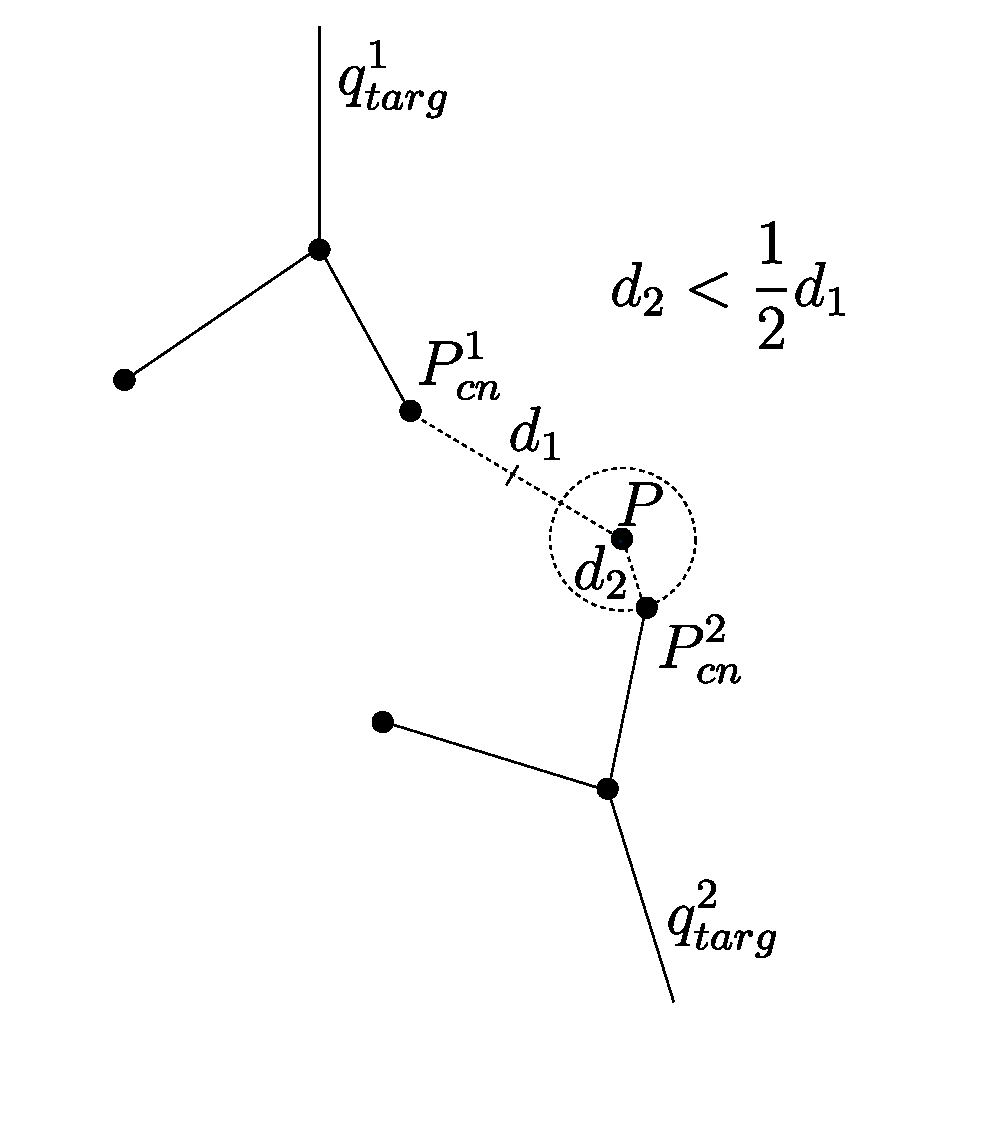
\includegraphics[scale=0.4]{figuras/competing-optimized-arterial-trees/exemplo-construcao-diagrama-voronoi-a.pdf}}
  \hspace{12pt}
  \subfloat[][]{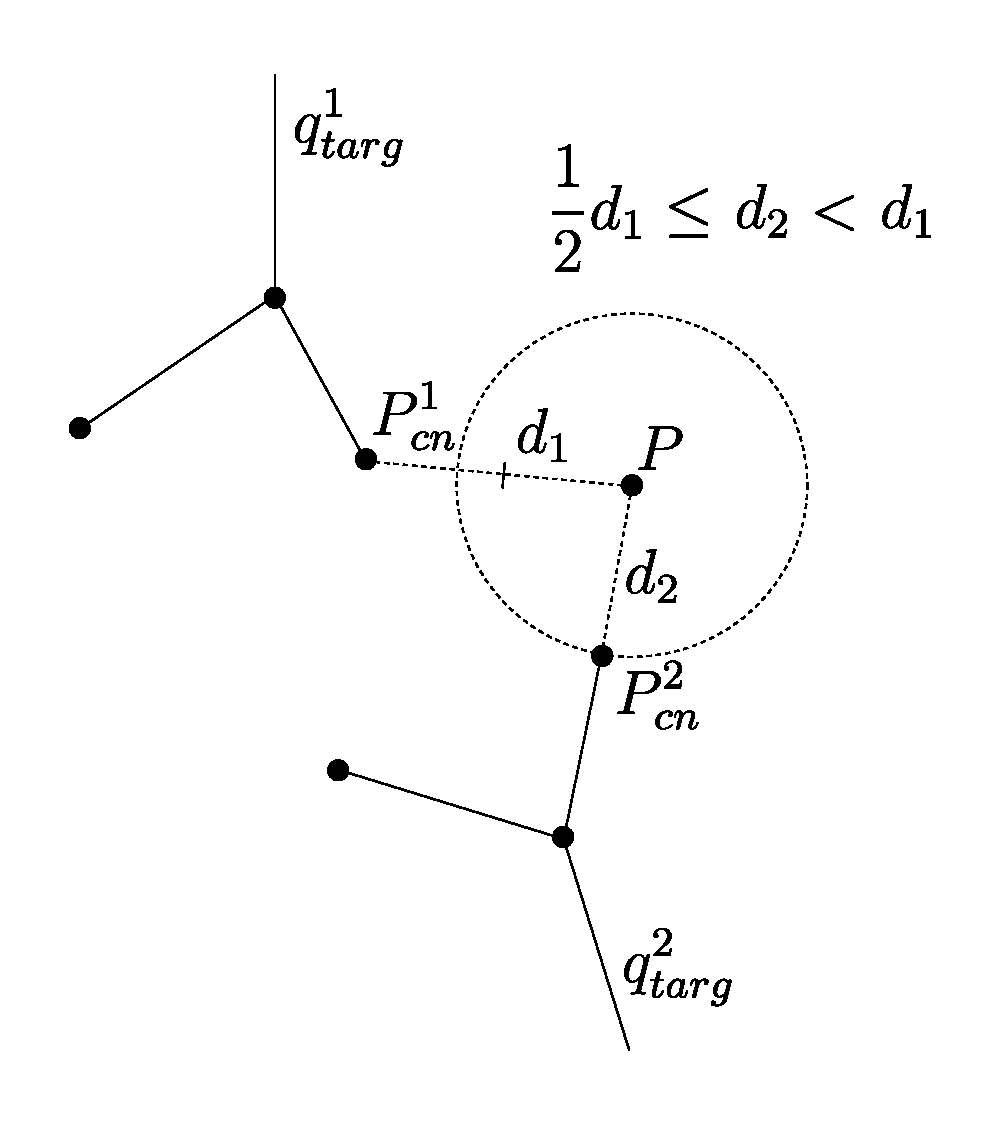
\includegraphics[scale=0.4]{figuras/competing-optimized-arterial-trees/exemplo-construcao-diagrama-voronoi-b.pdf}}

  \fonteAutor{2022}\label{fig:exemplo-construcao-diagrama-voronoi}
\end{figure}

\subsection{Construção da floresta no segundo estágio}\label{subsec:construcao-da-floresta-segundo-estagio}

No segundo estágio, cada árvore $t$ continua o seu crescimento. Admite-se o 
ponto $\mathbf{x}_{inew}$ como posição distal de um novo segmento terminal
se ele atender as condições:
\begin{enumerate}[label=(\Roman*)]
 \item estiver dentro do subdomínio $D_t$;
 \item sua distância a todos os segmentos da árvore $t$ for maior do que 
 $d_{min}^t$ (conforme definido em ~\eqref{eq:distancia-minima});
\end{enumerate}

\begin{algorithm}
\Dados{
  $D_{perf}$, $\mathbf{x}_{root}^t$, $q_{targ}^t$, 
  $N_{term}$, $N_{trees}$, $\alpha$, $N_{con}$, 
  $\beta$, $\eta$, $\lambda$.
}

  \textit{\underline{Primeiro estágio:}} abrir (ou construir) a floresta inicial\;
  Dividir $D_{perf}$ em subdomínios disjuntos $D_1$, $D_2$, \ldots, $D_{N_{trees}}$\;
  $K_{term}\leftarrow$ número atual de segmentos terminais na floresta\;
  \textit{\underline{Segundo estágio:}}
  \While{($K_{term} < N_{term}$)}{
    Gerar a posi\c{c}\~ao distal $\mathbf{x}_{inew}$ e verificar a qual subdomínio $D_i$
    ela pertence\;
    Verificar as condições (I) e (II) para $\mathbf{x}_{inew}$\;
    Determinar $N \leq N_{con}$ segmentos que estão mais próximos de $\mathbf{x}_{inew}$ na 
    árvore $i$\;
    \For{($j\gets 0$ \KwTo N)}{
      Conectar $\mathbf{x}_{inew}$ temporariamente no segmento $j$, 
      criando a bifurca\c{c}\~ao $\mathbf{x}_{ibif}$\;
      Otimizar e validar a posi\c{c}\~ao de $\mathbf{x}_{ibif}$\;    
      Armazenar resultados de $\mathbf{x}_{ibif}$ na TAC\;
      Descartar conexão temporária $\mathbf{x}_{ibif}$\;
    }
    Obter a TAC$_r$ a partir de TAC removendo as conexões inválidas\;
    Determinar em TAC$_r$ a bifurcação ótima $\mathbf{x}_{iopt}$\;
    Conectar $\mathbf{x}_{inew}$ a $\mathbf{x}_{iopt}$ de modo permanente\;
	$K_{term}\gets K_{term} + 1$\;
  }
\caption{Gera\c{c}ão de floresta de árvores vasculares pelo COAT.}
\label{algo:COAT}
\end{algorithm}

O critério de distância presente nas 
condições (iii) e (II) pode ser muito restritivo e o processo aleatório de geração de 
$\mathbf{x}_{inew}$ pode ser repetido muitas vezes. Para relaxar esse critério, 
se a geração de $\mathbf{x}_{inew}$ for repetida $N_{toss}$ vezes sem conseguir 
obter uma posição que atenda (iii) (ou (II)), então $d_{min}$ será atualizado como 
$\beta d_{min}$, onde $\beta\in (0,\,1)$ é um fator de redução. Além disso, 
$d_{min}$ também será atualizado se por $N_{toss}$ vezes a posição atender 
(iii) (ou (II)), mas não for possível obter uma bifurcação ótima $\mathbf{x}_{iopt}$.
